% Hidden in the LyX source (LyX Note) and never printed in the thesis.
% Moved here from appendix/appendix.tex during the LyX-to-TeX conversion.
\begin{center}
\begin{table}[htbp]
\centering{}\centering 
\global\long\def\sym#1{\ifmmode^{#1}\else$^{#1}$\fi}%
 \caption{Unconditional Quantile Regression Coefficients on Log Wages}
\noindent\resizebox{\textwidth}{!}{%
\begin{tabular}{lcccc}
\toprule 
 & Variance &  & Gini & \tabularnewline
\cmidrule{2-5} \cmidrule{3-5} \cmidrule{4-5} \cmidrule{5-5} 
 & \multicolumn{1}{c}{2004/06} & \multicolumn{1}{c}{2011/12} & \multicolumn{1}{c}{2004/06} & \multicolumn{1}{c}{2011/12}\tabularnewline
RTI & 0.093\sym{{*}{*}{*}} & 1.216\sym{{*}{*}{*}} & 0.059\sym{{*}{*}{*}} & 0.669\sym{{*}{*}{*}}\tabularnewline
 & (0.005) & (0.023) & (0.002) & (0.011)\tabularnewline
Abstract & 0.080\sym{{*}{*}{*}} & 0.769\sym{{*}{*}{*}} & 0.027\sym{{*}{*}{*}} & 0.415\sym{{*}{*}{*}}\tabularnewline
 & (0.004) & (0.014) & (0.002) & (0.007)\tabularnewline
Routine & -0.052\sym{{*}{*}{*}} & -0.931\sym{{*}{*}{*}} & -0.034\sym{{*}{*}{*}} & -0.509\sym{{*}{*}{*}}\tabularnewline
 & (0.006) & (0.019) & (0.003) & (0.009)\tabularnewline
Manual & 0.056\sym{{*}{*}{*}} & 1.166\sym{{*}{*}{*}} & 0.042\sym{{*}{*}{*}} & 0.640\sym{{*}{*}{*}}\tabularnewline
 & (0.006) & (0.023) & (0.003) & (0.011)\tabularnewline
Non-Married & 0.075\sym{{*}{*}{*}} & 0.051\sym{{*}{*}{*}} & 0.032\sym{{*}{*}{*}} & 0.019\sym{{*}{*}{*}}\tabularnewline
 & (0.002) & (0.002) & (0.001) & (0.001)\tabularnewline
Part-time & 0.363\sym{{*}{*}{*}} & 0.532\sym{{*}{*}{*}} & 0.098\sym{{*}{*}{*}} & 0.148\sym{{*}{*}{*}}\tabularnewline
 & (0.008) & (0.006) & (0.004) & (0.003)\tabularnewline
Non-permanent & 0.182\sym{{*}{*}{*}} & 0.171\sym{{*}{*}{*}} & 0.053\sym{{*}{*}{*}} & 0.054\sym{{*}{*}{*}}\tabularnewline
 & (0.005) & (0.004) & (0.002) & (0.002)\tabularnewline
Below Prim & 0.117\sym{{*}{*}{*}} & 0.039\sym{{*}{*}{*}} & 0.050\sym{{*}{*}{*}} & 0.025\sym{{*}{*}{*}}\tabularnewline
 & (0.005) & (0.005) & (0.002) & (0.002)\tabularnewline
High School & -0.020\sym{{*}{*}{*}} & -0.049\sym{{*}{*}{*}} & -0.011\sym{{*}{*}{*}} & -0.021\sym{{*}{*}{*}}\tabularnewline
 & (0.003) & (0.002) & (0.001) & (0.001)\tabularnewline
College & 0.098\sym{{*}{*}{*}} & 0.084\sym{{*}{*}{*}} & 0.050\sym{{*}{*}{*}} & 0.044\sym{{*}{*}{*}}\tabularnewline
 & (0.004) & (0.003) & (0.002) & (0.002)\tabularnewline
6-10 yrs & 0.004 & 0.006\sym{*} & -0.009\sym{{*}{*}{*}} & -0.004\sym{{*}{*}{*}}\tabularnewline
 & (0.003) & (0.003) & (0.001) & (0.001)\tabularnewline
11-15 yrs & 0.041\sym{{*}{*}{*}} & 0.063\sym{{*}{*}{*}} & 0.002 & 0.014\sym{{*}{*}{*}}\tabularnewline
 & (0.003) & (0.003) & (0.002) & (0.002)\tabularnewline
16-20 yrs & 0.085\sym{{*}{*}{*}} & 0.113\sym{{*}{*}{*}} & 0.018\sym{{*}{*}{*}} & 0.035\sym{{*}{*}{*}}\tabularnewline
 & (0.004) & (0.004) & (0.002) & (0.002)\tabularnewline
21-25 yrs & 0.108\sym{{*}{*}{*}} & 0.142\sym{{*}{*}{*}} & 0.027\sym{{*}{*}{*}} & 0.044\sym{{*}{*}{*}}\tabularnewline
 & (0.005) & (0.005) & (0.002) & (0.002)\tabularnewline
26-30 yrs & 0.110\sym{{*}{*}{*}} & 0.168\sym{{*}{*}{*}} & 0.035\sym{{*}{*}{*}} & 0.059\sym{{*}{*}{*}}\tabularnewline
 & (0.008) & (0.007) & (0.003) & (0.003)\tabularnewline
> 30 yrs & 0.121\sym{{*}{*}{*}} & 0.156\sym{{*}{*}{*}} & 0.045\sym{{*}{*}{*}} & 0.061\sym{{*}{*}{*}}\tabularnewline
 & (0.010) & (0.009) & (0.004) & (0.004)\tabularnewline
Managers & 0.236\sym{{*}{*}{*}} & 0.312\sym{{*}{*}{*}} & 0.171\sym{{*}{*}{*}} & 0.166\sym{{*}{*}{*}}\tabularnewline
 & (0.016) & (0.014) & (0.007) & (0.006)\tabularnewline
Professionals & 0.065\sym{{*}{*}{*}} & 0.159\sym{{*}{*}{*}} & 0.074\sym{{*}{*}{*}} & 0.078\sym{{*}{*}{*}}\tabularnewline
 & (0.015) & (0.012) & (0.007) & (0.006)\tabularnewline
Technicians & 0.012 & 0.007 & 0.026\sym{{*}{*}{*}} & -0.019\sym{{*}{*}{*}}\tabularnewline
 & (0.010) & (0.008) & (0.004) & (0.004)\tabularnewline
Clerks & 0.021 & -0.275\sym{{*}{*}{*}} & 0.016\sym{{*}{*}{*}} & -0.180\sym{{*}{*}{*}}\tabularnewline
 & (0.011) & (0.007) & (0.005) & (0.003)\tabularnewline
Services \& Sales Workers & 0.103\sym{{*}{*}{*}} & 0.212\sym{{*}{*}{*}} & 0.053\sym{{*}{*}{*}} & 0.103\sym{{*}{*}{*}}\tabularnewline
 & (0.006) & (0.005) & (0.003) & (0.003)\tabularnewline
Craft \& Trade Workers & -0.061\sym{{*}{*}{*}} & -0.049\sym{{*}{*}{*}} & -0.050\sym{{*}{*}{*}} & -0.044\sym{{*}{*}{*}}\tabularnewline
 & (0.005) & (0.004) & (0.002) & (0.002)\tabularnewline
Machine Operators & -0.049\sym{{*}{*}{*}} & -0.180\sym{{*}{*}{*}} & -0.040\sym{{*}{*}{*}} & -0.115\sym{{*}{*}{*}}\tabularnewline
 & (0.005) & (0.005) & (0.002) & (0.002)\tabularnewline
Constant & 0.220\sym{{*}{*}{*}} & 0.189\sym{{*}{*}{*}} & 0.272\sym{{*}{*}{*}} & 0.276\sym{{*}{*}{*}}\tabularnewline
 & (0.005) & (0.004) & (0.002) & (0.002)\tabularnewline
Observations & 198740 & 180656 & 198740 & 180656\tabularnewline
Adjusted $R^{2}$ & 0.113 & 0.192 & 0.097 & 0.165\tabularnewline
\bottomrule
\end{tabular}}
\end{table}
\begin{sidewaystable}[H]
\caption{Regression models for the college-high school log wage gap, 2004-2020}

\begin{centering}
\begin{tabular}{lccccc}
\toprule 
 & 2004-2012 &  & 2004-2020 &  & \tabularnewline
 & (1) & (2) & (3) & (4) & (5)\tabularnewline
\midrule
CLG/HS relative supply & 0.08273 & 0.48033 & 0.00454 & 0.04505 & -0.06677\tabularnewline
 & (0.261) & (0.286) & (0.137) & (0.105) & (0.118)\tabularnewline
Time & 0.00344 & -0.03359{*} & 0.00977 & 0.02172{*}{*} & 0.04206{*}{*}\tabularnewline
 & (0.019) & (0.018) & (0.010) & (0.008) & (0.014)\tabularnewline
Time X post-2012 &  &  & -0.02615{*}{*}{*} &  & \tabularnewline
 &  &  & (0.003) &  & \tabularnewline
Time$^{2}$/100 &  &  &  & -0.15331{*}{*}{*} & -0.32309{*}{*}{*}\tabularnewline
 &  &  &  & (0.015) & (0.101)\tabularnewline
Time$^{3}$/1000 &  &  &  &  & 0.06060\tabularnewline
 &  &  &  &  & (0.036)\tabularnewline
Constant & 0.51936 & 1.06468{*}{*}{*} & 0.41824{*}{*} & 0.44288{*}{*}{*} & 0.28137{*}\tabularnewline
 & (0.330) & (0.351) & (0.172) & (0.132) & (0.156)\tabularnewline
Observations & 9 & 17 & 17 & 17 & 17\tabularnewline
R-squared & 0.686 & 0.294 & 0.878 & 0.925 & 0.940\tabularnewline
\bottomrule
\end{tabular}
\par\end{centering}
Standard errors in parentheses{*}{*}{*} p<0.01, {*}{*} p<0.05, {*}
p<0.1
\end{sidewaystable}
\begin{table}[H]
\caption{}

\centering{}%
\begin{tabular}{cccccc}
\toprule 
 & logwage & abstract & routine & manual & RTI\tabularnewline
\midrule
logwage & 1 &  &  &  & \tabularnewline
abstract & 0.3914 & 1 &  &  & \tabularnewline
routine & -0.1186 & -0.5879 & 1 &  & \tabularnewline
manual & -0.2190 & -0.5172 & 0.5285 & 1 & \tabularnewline
RTI & -0.2674 & -0.8798 & 0.7828 & 0.2746 & 1\tabularnewline
\bottomrule
\end{tabular}
\end{table}
\begin{sidewaystable}[H]
\caption{}

\centering{}\noindent\resizebox{\textwidth}{!}{%
\begin{tabular}{ccccccccccccc}
\toprule 
 & logwage & nr\_cog\_anal & nr\_cog\_pers & r\_cog & r\_man & nr\_man\_phys & nr\_man\_pers & offshor & abstract & routine & manual & rti\tabularnewline
\midrule
logwage & 1 &  &  &  &  &  &  &  &  &  &  & \tabularnewline
nr\_cog\_anal & 0.403636461 & 1 &  &  &  &  &  &  &  &  &  & \tabularnewline
nr\_cog\_pers & 0.357828795 & 0.886646933 & 1 &  &  &  &  &  &  &  &  & \tabularnewline
r\_cog & 0.072768638 & -0.09819481 & 0.005465951 & 1 &  &  &  &  &  &  &  & \tabularnewline
r\_man & -0.211206291 & -0.786430687 & -0.724802192 & 0.342063432 & 1 &  &  &  &  &  &  & \tabularnewline
nr\_man\_phys & -0.260889227 & -0.757715762 & -0.651612844 & 0.053622539 & 0.845820079 & 1 &  &  &  &  &  & \tabularnewline
nr\_man\_pers & 0.250356442 & 0.798531165 & 0.894815847 & -0.036667414 & -0.848077041 & -0.757864663 & 1 &  &  &  &  & \tabularnewline
offshor & -0.068335603 & -0.164189917 & -0.349888515 & 0.074763906 & -0.007266434 & -0.276018921 & -0.25113619 & 1 &  &  &  & \tabularnewline
abstract & 0.391455014 & 0.969891526 & 0.972574448 & -0.046509445 & -0.777243051 & -0.724257084 & 0.872862973 & -0.266841697 & 1 &  &  & \tabularnewline
routine & -0.118693788 & -0.619453184 & -0.524767665 & 0.729718774 & 0.892111723 & 0.641236092 & -0.634726035 & 0.03066063 & -0.587916559 & 1 &  & \tabularnewline
manual & -0.219065329 & -0.599754877 & -0.409428728 & 0.052584124 & 0.691620946 & 0.942789636 & -0.497000544 & -0.495456016 & -0.51726843 & 0.528535177 & 1 & \tabularnewline
rti & -0.267493082 & -0.835587902 & -0.87264747 & 0.400347225 & 0.811303253 & 0.52804793 & -0.837018934 & 0.431667506 & -0.87982652 & 0.782832242 & 0.27461408 & 1\tabularnewline
\bottomrule
\end{tabular}}
\end{sidewaystable}
\begin{figure}[H]
\caption{KM predicted vs observed}

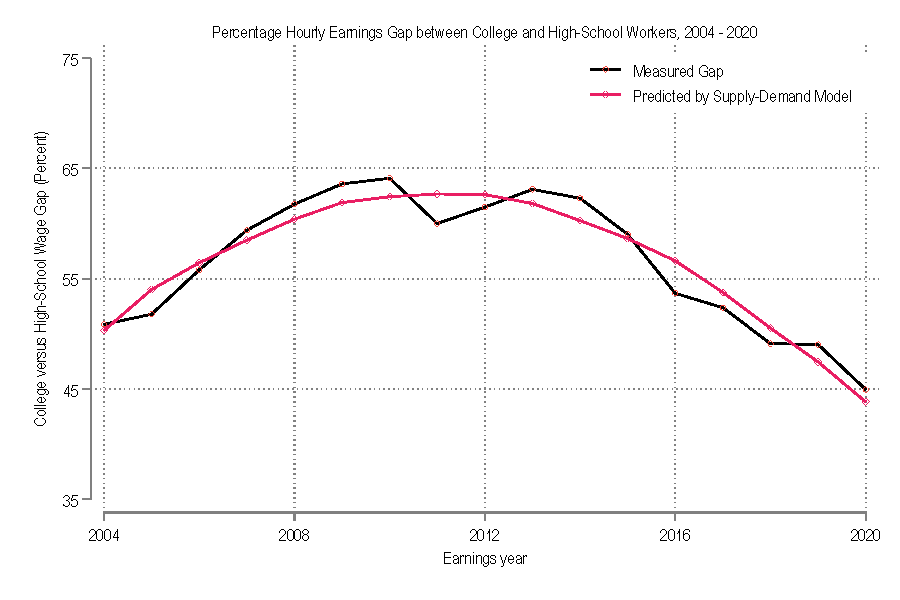
\includegraphics{extras/figs-hidden/km-quadratic-2004-2020.pdf}
\end{figure}
\begin{figure}[H]
\begin{singlespace}
\caption{Fitted Values}

\end{singlespace}
\begin{centering}
\subfloat[2004-2012]{\centering{}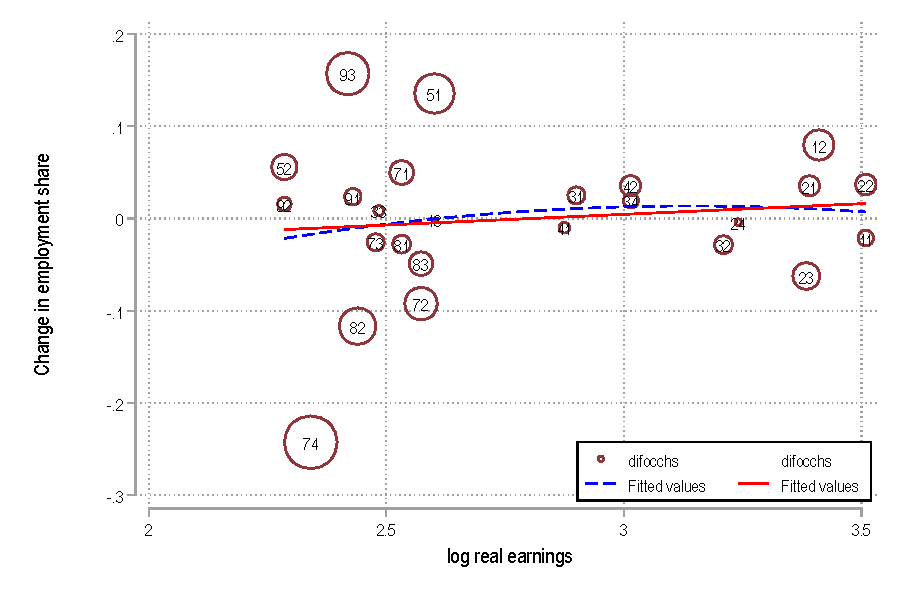
\includegraphics[width=0.5\textwidth]{extras/figs-hidden/regressed-polarization-emp-2004-2012.pdf}}\subfloat[]{\centering{}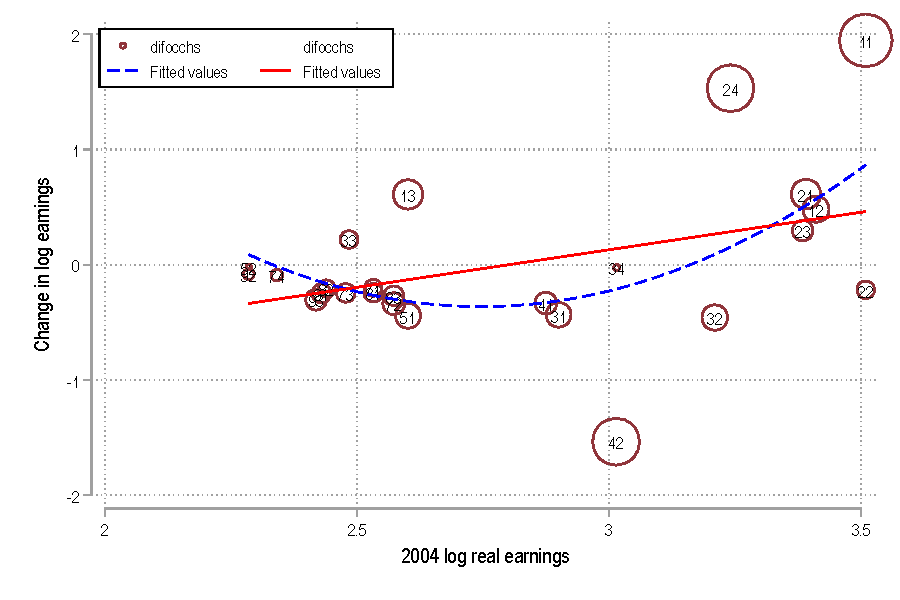
\includegraphics[width=0.5\textwidth]{extras/figs-hidden/regressed-polarization-wage-2004-2012.pdf}}
\par\end{centering}
\begin{centering}
\subfloat[]{\centering{}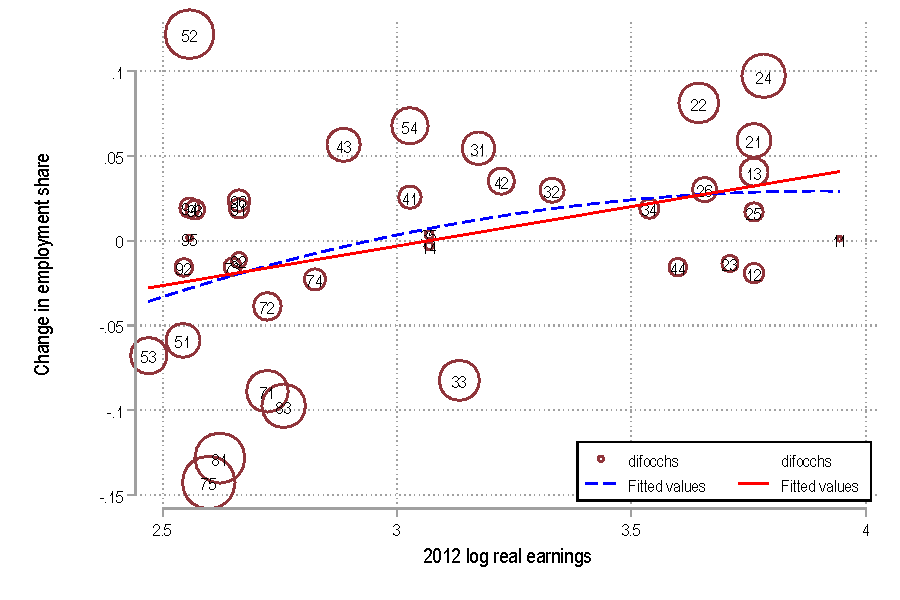
\includegraphics[width=0.5\textwidth]{extras/figs-hidden/regressed-polarization-emp-2012-2020.pdf}}\subfloat[]{\centering{}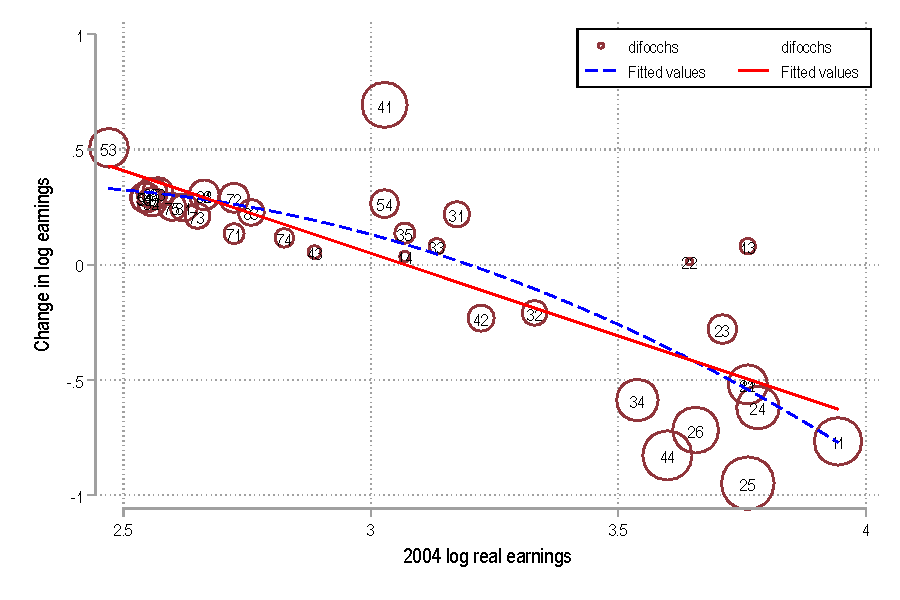
\includegraphics[width=0.5\textwidth]{extras/figs-hidden/regressed-polarization-wage-2012-2020.pdf}}
\par\end{centering}
\centering{}\subfloat[]{\centering{}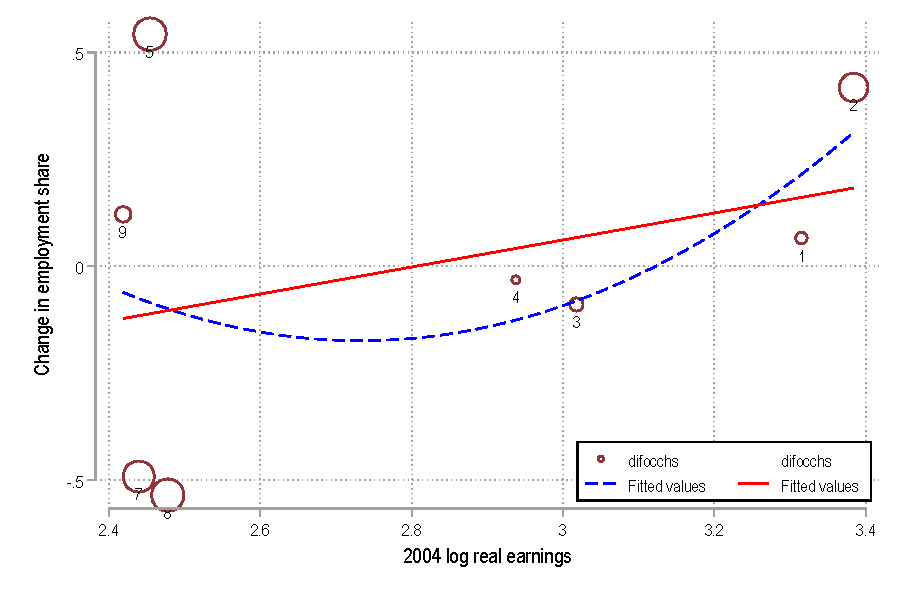
\includegraphics[width=0.5\textwidth]{extras/figs-hidden/regressed-polarization-emp-2004-2020.pdf}}\subfloat[]{\centering{}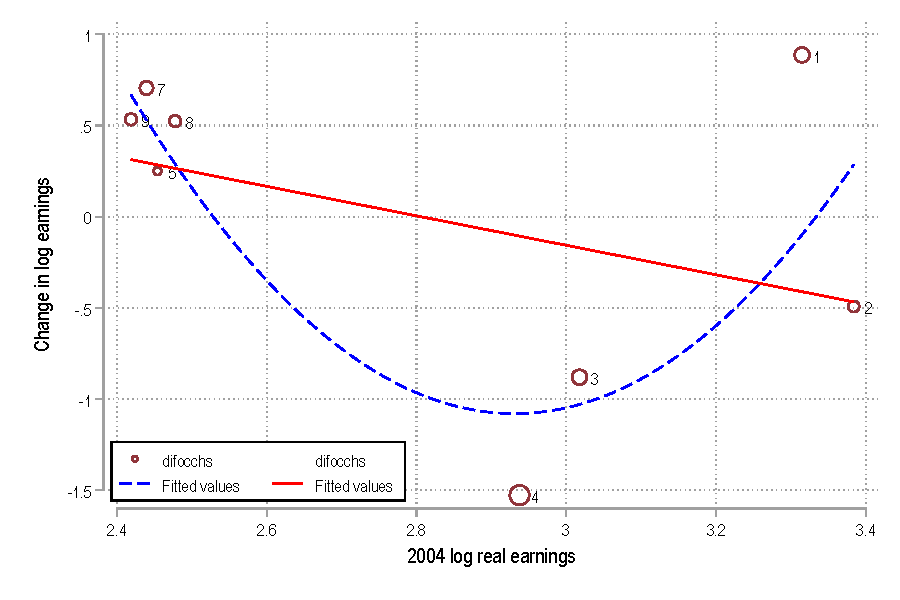
\includegraphics[width=0.5\textwidth]{extras/figs-hidden/regressed-polarization-wage-2004-2020.pdf}}
\end{figure}
\begin{table}[H]
\begin{onehalfspace}
\caption{Correlation Table}

\end{onehalfspace}
\centering{}\noindent\resizebox{\textwidth}{!}{%
\begin{tabular}{>{\raggedright}p{2cm}>{\raggedleft}p{1.5cm}@{\extracolsep{0pt}.}p{1.5cm}>{\centering}p{3cm}>{\centering}p{2cm}>{\centering}p{2cm}>{\centering}p{2cm}>{\centering}p{2cm}}
\toprule 
 & \multicolumn{7}{c}{2004}\tabularnewline
 & NR Cog& Analytical & NR Cog. Personal & R. Cog & R. Manual & Manual & wage\tabularnewline
 & \multicolumn{2}{p{3cm}}{} &  &  &  &  & \tabularnewline
NR Cog. Analytical & \multicolumn{2}{p{3cm}}{1} &  &  &  &  & \tabularnewline
NR Cog. Personal & 0&81 & 1 &  &  &  & \tabularnewline
R. Cog & -0&09 & 0.13 & 1 &  &  & \tabularnewline
R. Manual & -0&78 & -0.55 & 0.47 & 1 &  & \tabularnewline
Manual & -0&02 & 0.35 & 0.21 & 0.11 & 1 & \tabularnewline
Wage & 0&77 & 0.84 & 0.22 & -0.37 & 0.06 & 1\tabularnewline
\midrule 
 & \multicolumn{7}{c}{2012}\tabularnewline
NR Cog. Analytical & 1&00 &  &  &  &  & \tabularnewline
NR Cog. Personal & 0&70 & 1 &  &  &  & \tabularnewline
R. Cog & -0&11 & -0.55 & 1 &  &  & \tabularnewline
R. Manual & -0&60 & -0.77 & 0.52 & 1 &  & \tabularnewline
Manual & 0&16 & 0.50 & -0.30 & -0.03 & 1 & \tabularnewline
Wage & 0&87 & 0.66 & -0.09 & -0.65 & 0.03 & 1\tabularnewline
\bottomrule
\end{tabular}}
\end{table}
\begin{figure}[H]
\begin{centering}
\ContinuedFloat\caption{(continued)}
\subfloat[Males]{\centering{}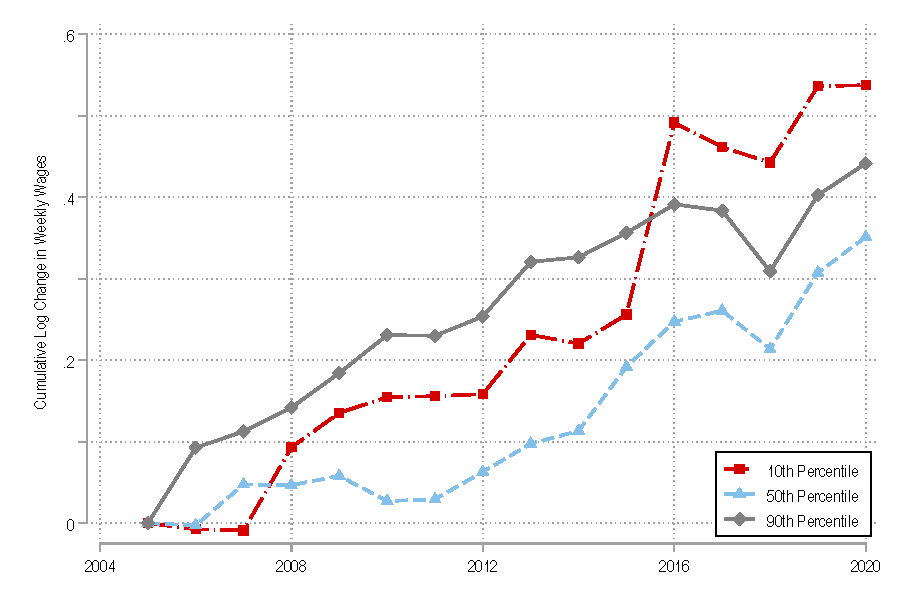
\includegraphics[width=1\textwidth]{extras/figs-hidden/wage-percentiles-90-50-10-m.pdf}}
\par\end{centering}
\centering{}\subfloat[Males and Females]{\centering{}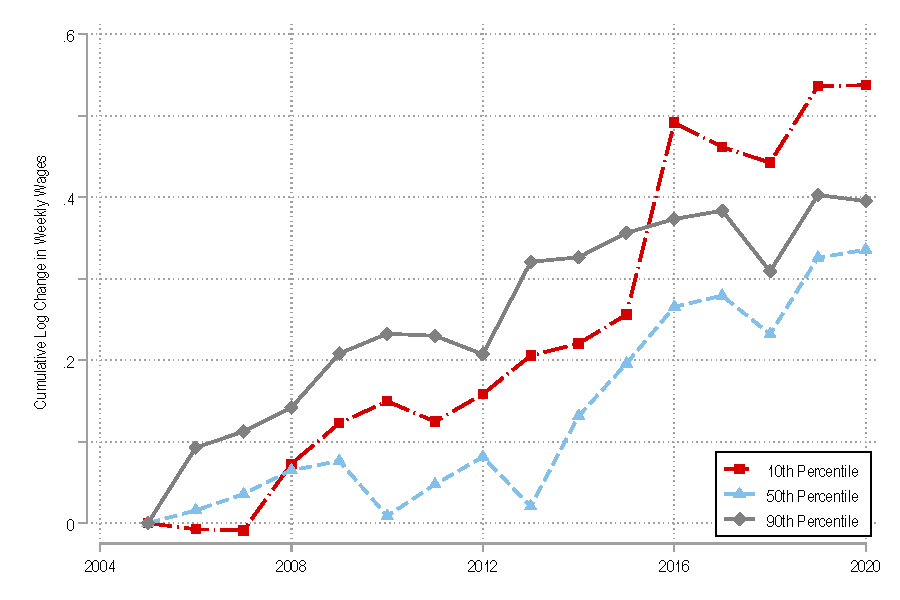
\includegraphics[width=1\textwidth]{figs/ch2/wage-percentiles-90-50-10-mf.pdf}}
\end{figure}
\par\end{center}
